% nt-01-narrative.tex

\documentclass[xcolor=dvipsnames]{beamer}
\usepackage{teachbeamer}

\title{Narrative Identity}
\subtitle{{\CourseNumber}, {\CourseInst}}

\author{\CourseName}

\date{May 15, 2018}

\begin{document}

\begin{frame}
  \titlepage
\end{frame}

\begin{frame}
  \frametitle{Nietzsche Introduction}
  \begin{block}{Gay Science, 124}
    We have left the land and have gone aboard ship! We have broken
    down the bridge behind us, nay, more, the land behind us! Well,
    little ship! Look out! Beside you is the ocean; it is true it
    does not always roar, and sometimes it spreads out like silk and
    gold and a gentle reverie. But times will come when you will feel
    that it is infinite, and that there is nothing more frightful than
    infinity. Oh, the poor bird that felt itself free and now strikes
    against the walls of this cage! Alas, if homesickness for the
    land should attack you, as if there had been more freedom there,
    and there is no ``land'' any longer!
  \end{block}
\end{frame}

% \begin{frame}
%   \frametitle{iClicker Question}
% Choose from the following options. This item will be graded.
% \begin{block}{iClicker Question}
% [2584] What was the Sultan's reaction to being cuckolded in \emph{The Arabian
% Nights}?
% \end{block}
% \begin{description}
% \item[A\hspace{.2in}$\blacktriangleright$] spend each night with a virgin and slay her the next morning
% \item[D\hspace{.2in}$\blacktriangleright$] repeat the cuckolding narrative in a type of role play with his wives
% \item[B\hspace{.2in}$\blacktriangleright$] ban all love stories from his kingdom
% \item[C\hspace{.2in}$\blacktriangleright$] retreat to the mountains in eternal hatred of women
% \end{description}
% \end{frame}

% \begin{frame}
%   \frametitle{iClicker Question}
% Choose from the following options. This item will be graded.
% \begin{block}{iClicker Question}
% [7230] Whose apricot tree was the source of Rebecca Solnit's mountain of apricots?
% \end{block}
% \begin{description}
% \item[A\hspace{.2in}$\blacktriangleright$] her father's
% \item[B\hspace{.2in}$\blacktriangleright$] her wife's
% \item[C\hspace{.2in}$\blacktriangleright$] her mother's
% \item[D\hspace{.2in}$\blacktriangleright$] her grandmother's
% \end{description}
% \end{frame}

\begin{frame}
  \frametitle{The Role of Narrative}
Which of these adjective apply to the role of narrative in a person's
life?
\begin{itemize}
\item necessary
\item inescapable
\item immutable
\item flexible
\item justificatory
\end{itemize}
\end{frame}

\begin{frame}
  \frametitle{The Role of Narrative}
What is the relationship of narrative to these other concepts in its
conceptual neighbourhood?
\begin{itemize}
\item power
\item violence
\item silence
\item memory
\item coherence
\end{itemize}
\end{frame}

% \begin{frame}
%   \frametitle{iClicker Question}
% Choose from the following options. This item will not be graded.
% \begin{block}{iClicker Question}
% [2264] Which of the following features is not one that Galen Strawson
% investigates as a possible condition for diachronicity?
% \end{block}
% \begin{description}
% \item[A\hspace{.2in}$\blacktriangleright$] form-finding
% \item[B\hspace{.2in}$\blacktriangleright$] story-telling tendency
% \item[C\hspace{.2in}$\blacktriangleright$] journalling
% \item[D\hspace{.2in}$\blacktriangleright$] revision
% \end{description}
% \end{frame}

% \begin{frame}
%   \frametitle{iClicker Question}
% Choose from the following options. This item will not be graded.
% \begin{block}{iClicker Question}
% [1442] Who is Strawson's example of someone who thinks that the psychological
% narrativity thesis is true (ordinary human beings experience their
% lives in some sort of narrative way), but the ethical narrativity
% thesis is NOT true (the narrative outlook is not essential to a
% well-lived life)?
% \end{block}
% \begin{description}
% \item[A\hspace{.2in}$\blacktriangleright$] Henry James
% \item[B\hspace{.2in}$\blacktriangleright$] Jean-Paul Sartre
% \item[C\hspace{.2in}$\blacktriangleright$] Marya Schechtman
% \item[D\hspace{.2in}$\blacktriangleright$] Charles Taylor
% \end{description}
% \end{frame}

\begin{frame}
  \frametitle{Nietzsche on Narrativity}
  \begin{block}{Human, All Too Human, 255}
    The superstition of the simultaneous. Simultaneous things hold
    together, it is said. A relative dies far away, and at the same
    time we dream about him, Consequently! But countless relatives die
    and we do not dream about them. It is like shipwrecked people who
    make vows; afterwards, in the temples, we do not see the votive
    tablets of those who perished. 
  \end{block}
\end{frame}

\begin{frame}
  \frametitle{Nietzsche on Narrativity}
  \begin{block}{Human, All Too Human, 255}
    A man dies, an owl hoots, a clock stops, all at one hour of the
    night, must there not be some connection? Such an intimacy with
    nature as this supposition implies is flattering to mankind. This
    species of superstition is found again in a refined form in
    historians and delineators of culture, who usually have a kind of
    hydrophobic horror of all that senseless mixture in which
    individual and national life is so rich.
  \end{block}
\end{frame}

\begin{frame}
  \frametitle{Two Claims}
  \begin{description}
  \item[psychological thesis] this is a descriptive, empirical claim
    about the nature of ordinary human experience, where a lack of
    narrativity is pathological with respect to how ordinary that
    experience is
  \item[ethical thesis] this is a normative, ethical claim that a
    narrative outlook is essential to a well-lived life, to true or
    full personhood
  \end{description}
\end{frame}

\begin{frame}
  \frametitle{Combinations of the Two Claims}
  \begin{tabular}{|l|l|l|}\hline
    \hspace{.5in}               & \hspace{.5in}        & \hspace{.5in}  \\
                                & psychological thesis & ethical thesis \\
    \hspace{.5in}               & \hspace{.5in}        & \hspace{.5in}  \\ \hline
    \hspace{.5in}               & \hspace{.5in}        & \hspace{.5in} \\
    Sartre/Stoics               & yes                  & no             \\
    \hspace{.5in}               & \hspace{.5in}        & \hspace{.5in}  \\ \hline
    \hspace{.5in}               & \hspace{.5in}        & \hspace{.5in} \\
    Plutarch                    & no                   & yes            \\ 
    \hspace{.5in}               & \hspace{.5in}        & \hspace{.5in}  \\ \hline
    \hspace{.5in}               & \hspace{.5in}        & \hspace{.5in} \\
    Schechtman/Taylor/MacIntyre & yes                  & yes            \\ 
    \hspace{.5in}               & \hspace{.5in}        & \hspace{.5in}  \\ \hline
    \hspace{.5in}               & \hspace{.5in}        & \hspace{.5in} \\
    Strawson                    & no                   & no             \\ 
    \hspace{.5in}               & \hspace{.5in}        & \hspace{.5in}  \\ \hline
  \end{tabular}
\end{frame}

\begin{frame}
  \frametitle{Dangers of Narrativity}
  Strawson claims (429) that the narrativity thesis in its two forms
  \begin{itemize}
  \item hinders self-understanding
  \item closes down important avenues of thought
  \item impoverishes our grasp of ethical possibilities
  \item needlessly and wrongly distresses those who do not fit the
    model
  \item is potentially destructive in psychotherapeutic contexts
  \end{itemize}
\end{frame}

\begin{frame}
  \frametitle{Relevant Questions}
  \begin{description}
  \item[diachronic] one naturally figures oneself, considered as a
    self, as something that was there in the past and will be there in
    the future
  \item[episodic] one does not figure oneself, considered as a
    self, as something that was there in the past and will be there in
    the future
  \end{description}
  Diachronicity is necessary (but not sufficient) for narrativity.
\end{frame}

\begin{frame}
  \frametitle{Relevant Questions}
  \begin{itemize}
  \item What are persistence conditions?
  \item What is the difference between a human being and a subjectively
    experienced self?
  \item What is true about these intuitions: the chilling, empty
    deficiency of the Episodic life versus the macerated, clogged,
    excessively self-concerned, inauthentically second-order qualities
    of the Diachronic life?
  \item Does it make a difference to be explicitly or implicitly
    narrativizing?
  \end{itemize}
\end{frame}

\begin{frame}
  \frametitle{The Episodic Life}
  \begin{block}{Against Narrativity, page 433}
    I have absolutely no sense of my life as a narrative with form, or
    indeed as a narrative without form. Absolutely none. Nor do I have
    any great or special interest in my past. Nor do I have a great
    deal of concern for my future.
  \end{block}
\end{frame}

\begin{frame}
  \frametitle{More Relevant Questions}
  \begin{itemize}
  \item How is it that the from-the-inside quality of a memory can be
    detached from any sense that one is the subject of the remembered
    experience (434)?
  \item Does Strawson give a satisfying answer to what it is to have
    or be a self? Is there an abolition of selfhood lurking in the
    background? Who am I, and if so, how many? (Richard David Precht)
    See also \emph{The Ego Tunnel} by Thomas Metzinger or \emph{The
      Architecture of the Mind} by Peter Carruthers. What are the
    metaphysics of selfhood?
  \item How do you assess Strawson's argument that the ethical
    narrativity claim is associated with self-importance, religion,
    and narcissism (436f)?
  \end{itemize}
\end{frame}

\begin{frame}
  \frametitle{More Relevant Questions}
  \begin{itemize}
  \item Does the making coffee narrative scale up to larger narratives
    and propagate to higher levels; or is Strawson correct to call the
    narrativity claim about short-term plans trivial?
  \item Has Strawson addressed the problem that narrativists have with
    an invasive scientific anthopology? (See footnote 27.)
  \item How can a narrative be defined stringently? Note Strawson's
    emphasis on developmental, temporal unity and coherence.
  \item What does a personal relationship with an Episodic look like?
  \end{itemize}
\end{frame}

\begin{frame}
  \frametitle{Jacques Derrida I}
  \begin{quote}
    I understand that the question of the marriage vows was, this
    morning, considered interesting by some of you, the ``yes'' to the
    marriage, the performative ``yes'' -- ``I do'', ``I do''. This
    ``yes'' has to be repeated differently each time. If it's simply a
    record saying ``I do'' ``I do'' ``I do'' there is no fidelity. For
    this ``I do'' to be a renewed promise it has to be different each
    time, the same one and different. In order to follow the ``I do''
    today (before the priest), the ``idea'' of tomorrow should be the
    same and different {\ldots}
  \end{quote}
\end{frame}

\begin{frame}
  \frametitle{Jacques Derrida II}
  \begin{quote}
    {\ldots} They must follow one another and confirm themselves but,
    at the same time, be different. That's what the counter-signature
    is. Of course, even if I say to the same person ``I do'' tomorrow
    and after tomorrow, the fact that this ``I do'' is different, to
    some extent, means at the same time fidelity and betrayal. Indeed,
    it's a kind of perjury to say ``I do'' to someone. So that may be
    the paradox in the twin concepts of acoluthia and anacoluthon. You
    have to betray in order to be truthful. (Life After Theory, 10f)
  \end{quote}
\end{frame}

\begin{frame}
  \frametitle{Conditions of Narrativity}
  \begin{description}
  \item[diachronicity] I identify myself (the one who is the receiver
    of my subjective experiences) with the human being that I was in
    the past and that I will be in the future
  \item[form-finding] I seek for coherence, unity, and pattern in the
    temporal sequence events in my life
  \item[story-telling] I think of my life in recognizable literary
    genres
  \item[revision] I distort facts about my life so that they fit the
    kind of story that I want to tell about myself (444)
  \end{description}
\end{frame}

\begin{frame}
  \frametitle{Strawson's Shift}
  There is a marked shift on page 447 to a negative evaluation of
  narrativity. There appears to be some inconsistency between the
  pre-447 Strawson and the post-447 Strawson.
\end{frame}

\begin{frame}
  \frametitle{Nietzsche on Narrativity}
  \begin{block}{Gay Science, 277}
    For now the thought of a personal Providence first presents itself
    before us with its most persuasive force, and has the best of
    advocates, apparentness, in its favour, now when it is obvious
    that all and everything that happens to us always turns out for
    the best. The life of every day and of every hour seems to be
    anxious for nothing else but always to prove this proposition
    anew; let it be what it will, bad or good weather, the loss of a
    friend, a sickness, a calumny, the non receipt of a letter, the
    spraining of one's foot, a glance into a shop window, a counter
    argument, the opening of a book, a dream, a deception: it shows
    itself immediately, or very soon afterwards, as something "not
    permitted to be absent," it is full of profound significance and
    utility precisely for us!
  \end{block}
\end{frame}

\begin{frame}
  \frametitle{Nietzsche on Narrativity}
  \begin{block}{Gay Science, 277}
    Is there a more dangerous temptation to rid ourselves of the
    belief in the Gods of Epicurus, those careless, unknown Gods, and
    believe in some anxious and mean Divinity, who knows personally
    every little hair on our heads, and feels no disgust in rendering
    the most wretched services? Well I mean in spite of all this! We
    want to leave the Gods alone (and the serviceable genii likewise),
    and wish to content ourselves with the assumption that our own
    practical and theoretical skilfulness in explaining and suitably
    arranging events has now reached its highest point.
  \end{block}
\end{frame}

\begin{frame}
  \frametitle{Nietzsche on Narrativity}
  \begin{block}{Gay Science, 277}
    We do not want either to think too highly of this dexterity of our
    wisdom, when the wonderful harmony which results from playing on
    our instrument sometimes surprises us too much: a harmony which
    sounds too well for us to dare to ascribe it to ourselves. In
    fact, now and then there is one who plays with us beloved Chance:
    he leads our hand occasionally, and even the all wisest Providence
    could not devise any finer music than that of which our foolish
    hand is then capable.
  \end{block}
\end{frame}

% \begin{frame}
%   \frametitle{iClicker Question}
% Choose from the following options. This item will be graded.
% \begin{block}{iClicker Question}
% [7014] On the Non-Reductionist view, according to Derek Parfit in the reading for today,
% \end{block}
% \begin{description}
% \item[A\hspace{.2in}$\blacktriangleright$] moral choices cannot be reduced to calculations about consequences
% \item[B\hspace{.2in}$\blacktriangleright$] a person is a separately existing entity, distinct from brain, body, and experience
% \item[C\hspace{.2in}$\blacktriangleright$] moral questions cannot be reduced to scientific questions
% \item[D\hspace{.2in}$\blacktriangleright$] Buddha's message and the Judaeo-Christian message cannot be reduced to each other
% \end{description}
% \end{frame}

% \begin{frame}
%   \frametitle{iClicker Question}
% Choose from the following options. This item will be graded.
% \begin{block}{iClicker Question}
% [7859] According to Williams' two requirements, personal identity
% cannot depend on the following two features,
% \end{block}
% \begin{description}
% \item[A\hspace{.2in}$\blacktriangleright$] narrative and moral features
% \item[B\hspace{.2in}$\blacktriangleright$] episodic and diachronic features
% \item[C\hspace{.2in}$\blacktriangleright$] psychological and physical features
% \item[D\hspace{.2in}$\blacktriangleright$] non-intrinsic and trivial features
% \end{description}
% \end{frame}

\begin{frame}
  \frametitle{David Hume: Of Personal Identity}
  Hume's empiricism implies his (Parfit's term) reductionist view
  of the self. Since there are no simple and constant impressions
  of the self, there also can be no such idea.
  \begin{block}{David Hume}
    He may, perhaps, perceive something simple and continued,
    which he calls \emph{himself}; though I am certain there is no
    such principle in me. But setting aside some metaphysicians of
    this kind, I may venture to affirm of the rest of mankind,
    that they are nothing but a bundle or collection of different
    perceptions, which succeed each other with an inconceivable
    rapidity, and are in a perpetual flux and movement {\ldots}
    the mind is a kind of theatre (165)
  \end{block}
Like Strawson, Hume distinguishes between identity as it regards
our thought and imagination (Strawson's ``I$^{\ast}$'') and identity
as it regards our passions and concerns (Strawson's ``I''). 
\end{frame}

\begin{frame}
  \frametitle{David Hume: Of Personal Identity}
  \begin{block}{Hume, ``Of Personal Identity'' in \emph{A Treatise of Human Nature}}
    In this respect, I cannot compare the soul more properly to any
    thing than to a republic or commonwealth, in which the several
    members are united by the reciprocal ties of government and
    subordination, and give rise to other persons, who propagate the
    same republic in the incessant changes of its parts.
  \end{block}
\end{frame}

\begin{frame}
  \frametitle{Where Am I, Or What?}
  \begin{block}{David Hume}
    Where am I, or what? From what causes do I derive my
    existence, and to what condition shall I return? Whose favour
    shall I court, and whose anger must I dread? What beings
    surround me? And on whom have I any influence, or who have
    any influence on me? I am confounded with all these questions,
    and begin to fancy myself in the most deplorable condition
    imaginable, invironed with the deepest darkness, and utterly
    deprived of the use of every member and faculty. (175)
  \end{block}
\end{frame}

\begin{frame}
  \frametitle{Why Personal Identity Isn't What Matters}
  \begin{figure}[h]
    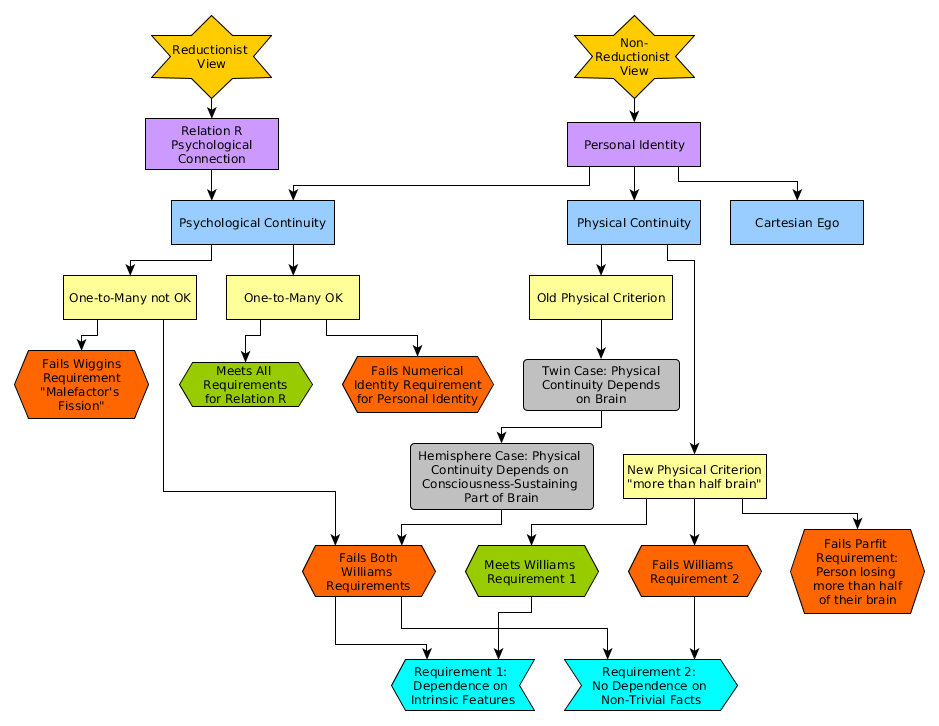
\includegraphics[scale=0.3]{./parfit.png}
  \end{figure}
\end{frame}

\begin{frame}
  \frametitle{Derek Parfit}
  \begin{quote}
    When I believed that my existence was a further fact, I seemed
    imprisoned in myself. My life seemed like a glass tunnel, through
    which I was moving faster every year, and at the end of which
    there was darkness. When I changed my view, the walls of my glass
    tunnel disappeared. I now live in the open air. (Derek Parfit,
    Reasons and Persons, 281)
  \end{quote}
\end{frame}

\begin{frame}
  \frametitle{John Stuart Mill}
  \begin{block}{Mill, \emph{Utilitarianism}}
    In an improving state of the human mind, the influences are
    constantly on the increase, which tend to generate in each
    individual a feeling of unity with all the rest; which, if
    perfect, would make him never think of, or desire, any beneficial
    condition for himself, in the benefits of which they are not
    included.
  \end{block}
\end{frame}

\begin{frame}
  \frametitle{Questions}
  \begin{itemize}
  \item Is Nagel's view correct that it is psychologically impossible
    to believe the Reductionist View? Is Parfit's view correct that we
    can believe the truth about ourselves (280)?
  \item Do you agree with Wittgenstein that counterfactuals do not
    elucidate concepts? (``Multiverse Ethics'')
  \item What are the psychological and moral effects of the
    Reductionist View on you?
  \item Do you agree with Nagel that with the expectation to be reset
    to an earlier state, you should summon your courage and prepare to
    die (compare the Hollywood movie \emph{Edge of Tomorrow})?
  \end{itemize}
\end{frame}

% \begin{frame}
%   \frametitle{iClicker Question}
% Choose from the following options. This item will be graded.
% \begin{block}{iClicker Question}
% [3515] For which philosopher's account of personal identity does Marya
% Schechtman point out that it rests on consciousness rather than, as
% usually assumed, memory?
% \end{block}
% \begin{description}
% \item[A\hspace{.2in}$\blacktriangleright$] John Locke
% \item[B\hspace{.2in}$\blacktriangleright$] David Hume
% \item[C\hspace{.2in}$\blacktriangleright$] J.S. Mill
% \item[D\hspace{.2in}$\blacktriangleright$] Immanuel Kant
% \end{description}
% \end{frame}

% \begin{frame}
%   \frametitle{iClicker Question}
% Choose from the following options. This item will be graded.
% \begin{block}{iClicker Question}
% [8240] Which of these are not part of a Schechtman illustration in her paper?
% \end{block}
% \begin{description}
% \item[A\hspace{.2in}$\blacktriangleright$] the fat lady in the picture
% \item[B\hspace{.2in}$\blacktriangleright$] the sing-song of old man kangaroo
% \item[C\hspace{.2in}$\blacktriangleright$] the man who thought he was Napoleon
% \item[D\hspace{.2in}$\blacktriangleright$] Dr. Bernheim's umbrella
% \end{description}
% \end{frame}

\begin{frame}
  \frametitle{Lanzmann versus Spielberg}
  Compare the following two film previews.
  \begin{alltt}
    https://www.youtube.com/watch?v=VXsgUnLG4CY
  \end{alltt}
  \begin{alltt}
    https://www.youtube.com/watch?v=JdRGC-w9syA
  \end{alltt}
\end{frame}

\begin{frame}
  \frametitle{The Four Features}
  Sentient beings and persons are distinguished by
  \begin{itemize}
  \item moral agency
  \item compensation
  \item self-interested concern
  \item survival
  \end{itemize}
  Individuals constitute themselves as persons by coming to think of
  themselves as persisting subjects who have had experience in the
  past and will continue to have experience in the future.
\end{frame}

\begin{frame}
  \frametitle{Constraints}
  \begin{description}
  \item[Articulation] Form and logic of a conventional, linear
    narrative. Constituents (characters, events) do not have a meaning
    on their own. Meaning comes from the configuration, from the plot.
    Time-slices are not fully intelligible. 
  \item[Reality] Self-constitution requires both an internal life and
    a proper connection to the social world. Self-conception must be
    in sync with that of others.
  \end{description}
  Mitigation of the ``no personhood without narrative'' claim: (i)
  other forms of existence are valuable; (ii) there is a wide
  diversity of qualifying narratives.
\end{frame}

\begin{frame}
  \frametitle{Parfit's Satori-Like Dissolution of the Self}
  Parfit concludes from the superficiality of psychological continuity
  that the self is a fiction. MS claims, however, that a Parfitian
  live-for-the-moment, sever-the-bonds-with-the-past-and-the-future
  life produces individuals who
  \begin{itemize}
  \item don't make plans
  \item don't engage in long-term commitments
  \item don't take responsibility for the past, and, in any case,
  \item don't embrace the concept of personhood
  \end{itemize}
  MS and DP only disagree on whether personhood is achievable without superficiality.
\end{frame}

\begin{frame}
  \frametitle{Marxist Concerns}
  A possible Marxist critique: the narrative self-constitution view is
  an insistence on conformity to the worldview of a dominant group. In
  response, Schechtman points out how much similarity there is between
  a revolutionary and a reactionary narrative compared to the contrast
  between a revolutionary narrative and the incoherence of a psychotic.
\end{frame}

\begin{frame}
  \frametitle{John Locke's Account of Personal Identity}
  Sameness of consciousness, not sameness of substance (Kafka's
  \emph{Metamorphosis}). The problem with a pure memory account of
  personal identity is that memories are by definition remembered,
  while consciousness can be affected more globally and partly
  subconsciously. Example: financial security.
\end{frame}

\begin{frame}
  \frametitle{Confabulation and Self-Blindness}
  Schechtman claims that to the extent to which we confabulate and
  deceive ourselves, our personhood is compromised. Umbrella episode
  with Dr.\ Bernheim. Heidegger/Habermas debate: does mysticism and
  ineffability enhance or reduce personhood?

  \bigskip

  Loss of personhood can also originate in not inhabiting the same
  world as one's fellows. MS puts much greater emphasis here on
  coherence of facts rather than coherence of interpretation (what
  about the first secular atheist, the psychopath, or the
  depressive?). 
\end{frame}

\begin{frame}
  \frametitle{Polyjuice Potion}
  Schechtman also claims that the narrative self-constitution view can
  mediate between two opposing views on continuity, the bodily vs the
  psychological continuity view. While the narrative self-constitution
  view is broadly supportive of the psychological view, it also
  underlines that the congress of body and person is not accidental.
\end{frame}

\end{document}
